% DO NOT COMPILE THIS FILE DIRECTLY!
% This is included by the other .tex files.

% Slide de t�tulo
\begin{frame}%[t,plain]
\titlepage

\note{Aqui voc� escreve o que vai falar durante este slide na apresenta��o.
}

\end{frame}


\begin{frame}{Outline}
  \tableofcontents
\end{frame}

% Se��o introdu��o
%******************************************************************
\section{Introdu��o}


%*OVERVIEW***********************************
\subsection{Vis�o Geral}


\begin{frame}{Vis�o Geral: Dados dispon�veis}


\begin{itemize}
	\item<1-5> As esta��es de pot�ncia sao conectadas por uma rede;
	\item<2-5> Dados do SCADA est�o dispon�veis;
	\item<3-5> Os dados dos reles de prote��o est�o dispon�veis;
	\item<4-5> E os dados do DFR (oscillography) podem tamb�m ser acessados.
	\item<5> Sincroniza��o com GPS baseada em tempo.
\end{itemize}
\vbox{}\vfill

\note{
I will start by giving an overview of what kinds of data are available nowadays in an analysis centre of a power generation utility.\\

go on, go on....

}

\end{frame}


\begin{frame}[t]{Defini��o do Problema}

\begin{itemize}
   \item Item 1 \pause
   \item Item 2 \pause
		\begin{itemize}
			\item subitem 1
			\item subitem 2 \pause
		\end{itemize}
  	\item Item 3

\end{itemize}

\onslide+{
\begin{beamercolorbox}[colsep=4pt,shadow=true,rounded=true,center]{title in head/foot}
{Uau!! This is an exclamation box, it is amazing!}
\end{beamercolorbox}
}

\note<1-3>{Notas para os slides 1 a 2.
}
\note<4-4>{Notas para os slides 3 a 4
}



\end{frame}



%*SUBSECTION***********************************
\subsection{Uma Subse��o}

\begin{frame}[t]{T�tulo}

\begin{itemize}
	\item Objetivo 1 \pause
	\item Objetivo 2 \pause
	\item Objetivo 3 \pause
	\item Objetivo 4
\end{itemize}


\note{Notas para este slide}

\end{frame}

%*SUBSECTION***********************************
\subsection{Outra Subse��o}

\begin{frame}[t]{Outro Slide}

\begin{figure}[!htb]
  \centering
  \mbox{%
    \subfloat[b][Mem�ria de Programa]{
    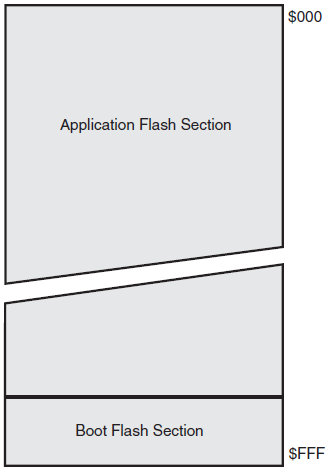
\includegraphics[height=5cm]{./figuras/avrprg.png}
    \label{fig:avr-prgmem}
    }
    \subfloat[b][Mem�ria de Dados]{
    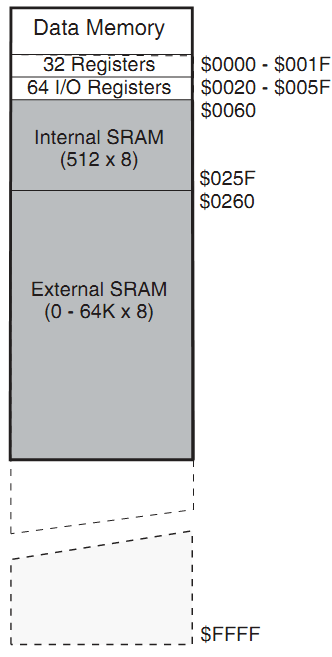
\includegraphics[height=5cm]{./figuras/avrdata.png}
    \label{fig:avr-datamem}
    }
   }
  \caption{Mapas de Mem�ria do AVR.}
  \label{fig:avr-memmap}
\end{figure}

\end{frame}

\begin{frame}[t]{Outro Slide, novamente}

\end{frame}

% SECTION
%******************************************************************
\section{Outra Se��o}

%*SUBSECTION***********************************
\subsection{Subse��o Novamente}


\begin{frame}[t]{T�tulo A}

\begin{lema}
fgfgfg
\end{lema}

\begin{teorema}
fsadfd
\end{teorema}

\begin{prova}
dfasdfa
\end{prova}

\begin{lema}
fgfgfg
\end{lema}


\end{frame}

\begin{frame}[t]{T�tulo B}

\end{frame}

\begin{frame}[t]{T�tulo C}

\end{frame}

%*SECTION***********************************
\section{Conclusions}

\begin{frame}[t]{Conclus�es}

Isto � apenas um exemplo.

\end{frame}




%*SECTION***********************************
\section{O Que Vem a Seguir?}

\begin{frame}[t]{Pr�ximo Passo}

Voc� pode come�ar sua pr�pria apresenta��o.

\end{frame}


%
\title{Obrigado!}
\begin{frame}[t,plain]{}

\titlepage
\end{frame} 